% author  Dinupa Nawarathne
% email  dinupa3@gmail.com
% date  10-01-2022


\documentclass{article}

% use packages
\usepackage{amsmath}
\usepackage{amssymb}
\usepackage{graphicx}
\usepackage[backend=bibtex, style=science]{biblatex}
\usepackage{hyperref}

% refs file
\addbibresource{refs.bib}

% title, author, date
\title{Gaussian Process Regression}
\author{Vassili Papavassiliou, \and Stephen Pate-Morales, \and Abinash Pun, \and Forhad Hossain, \and Dinupa Nawarathne, \and Harsha Kaluarachchi}
\date{October 01, 2022}

% document
\begin{document}

% title
\maketitle

% abstract
\begin{abstract}
Gaussian process regression (GPR) is a widely used learning technique in machine learning. Some of the basic concepts of Gaussian process (GP) are multivariate normal distributions, kernels and joint and conditional probability etc. In this note we explain the basic mathematics of GPR and one of the common library used in the python to make GPR predictions.
\end{abstract}

% Introduction
\section{Introduction}

The Gaussian process model is a probabilistic supervised machine learning technique used in classification and regression tasks. A Gaussian process regression (GPR) model can make predictions incorporating prior knowledge (kernels) and provide uncertainties of the predictions \cite{10.7551/mitpress/3206.001.0001}.

The advantages of the Gaussian process are \cite{scikit-learn};

\begin{itemize}
\item The prediction interpolates the observations (at least for regular kernels).
\item The prediction is probabilistic (Gaussian) so that one can compute empirical confidence intervals and decide based on those if one should refit (online fitting, adaptive fitting) the prediction in some region of interest.
\item Versatile: different kernels can be specified. Common kernels are provided, but it is also possible to specify custom kernels.
\end{itemize}

\section{Mathematical Basics}

Consider set of observed data points. We want to fit a function to represent these data points and then make a prediction at new data points. This is know as the regression. For a given set of observed data points, there are infinite number of possible functions that fit these data points. In GPR, Gaussian process conduct the regression by defining a distribution over these infinite number of functions.

\subsection{Gaussian Distribution}

A random variable $X$ is Gaussian or normally distributed with mean $\mu$ and variance $\sigma^{2}$ if its probability density function(PDF) is \cite{murphy2012machine};

\begin{equation}
P_{X}(x) = \frac{1}{\sqrt{2\pi}\sigma}\exp{-\frac{(x-\mu)^{2}}{2\sigma^{2}}}
\end{equation}

where $X$ is the random variables and $x$ is the real argument. The normal distribution of X is represented by;

\begin{equation}
P_{X} \sim \mathcal{N}(\mu, \sigma^{2})
\end{equation}

\begin{figure}
\centering
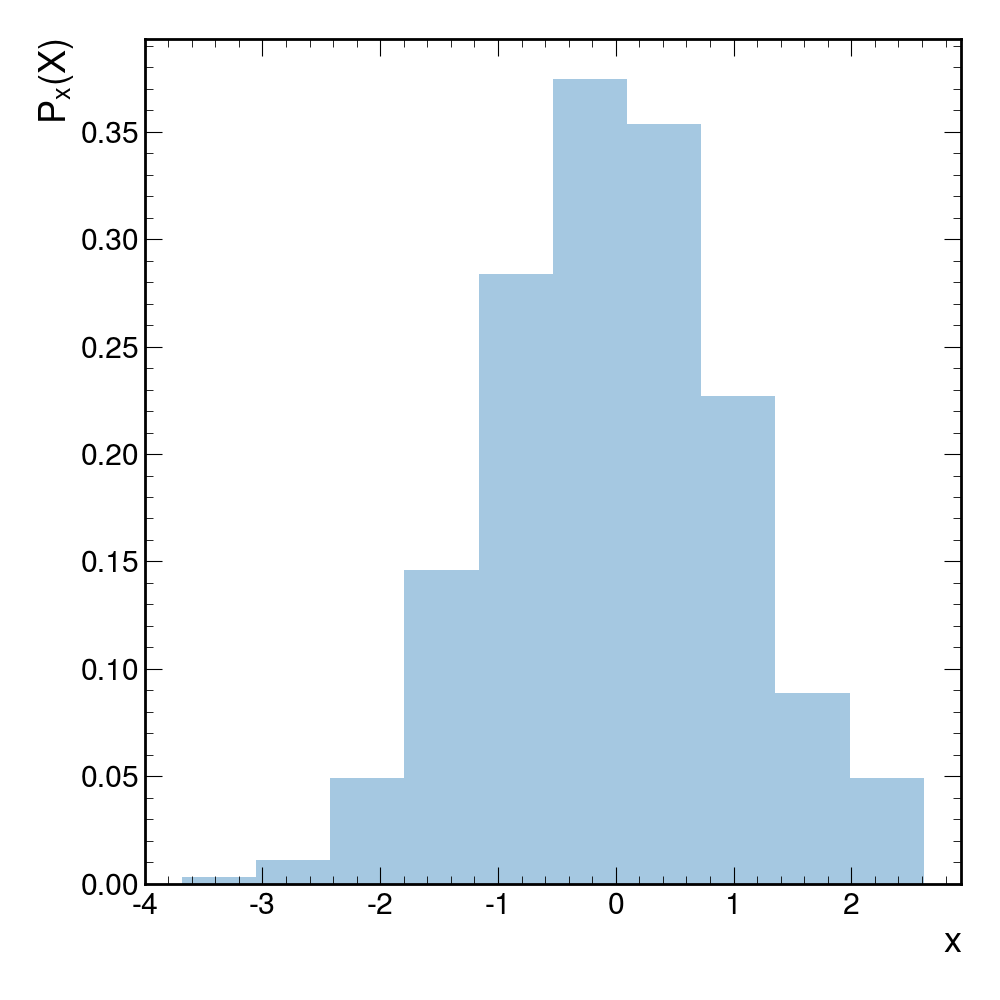
\includegraphics[width=8.0cm]{imgs/norm.png}
\caption{A uni-variate normal distribution for 1000 random points.}
\end{figure}

\subsection{Multivariate Normal Distribution}

The PDF of an multivariate normal distribution (MVN) with dimension $D$ is defined as \cite{murphy2012machine};

\begin{equation}
\mathcal{N}(x|\mu, \Sigma) = \frac{1}{(2\pi)^{\frac{D}{2}} |\Sigma|^{\frac{1}{2}}} \exp[{-\frac{1}{2}(x-\mu)^{T} \sigma^{-1}(x - \mu)}]
\end{equation}

where $D$ is the number of dimensions, $x$ is the variable, $\mu$ is the mean vector and $\Sigma$ is the covariance matrix. Consider the Gaussian random variable $y = \begin{bmatrix}
y_{1} \\
y_{2}
\end{bmatrix}$, mean $\mu = \begin{bmatrix}
\mu_{1} \\
\mu_{2}
\end{bmatrix}$ and covariance matrix $\Sigma = \begin{bmatrix}
\Sigma_{11} & \Sigma_{12} \\
\Sigma_{21} & \Sigma_{22}
\end{bmatrix}$. We have the following properties;

\begin{enumerate}
\item Normalization;

\begin{equation}
\int_{y} p(y; \mu, \Sigma) = 1
\end{equation}

\item Marginalization: The marginal distributions $p(y_{1}) = \int_{y_{2}} p(y_{1}, y_{2}; \mu, \Sigma) dy_{2}$ and $p(y_{2}) = \int_{y_{1}} p(y_{1}, y_{2}; \mu, \Sigma) dy_{1}$;

\begin{align}
y_{1} &\sim \mathcal{N}(\mu_{1}, \Sigma_{11}) \\
y_{2} &\sim \mathcal{N}(\mu_{2}, \Sigma_{22})
\end{align}

\item Summation: If $y_{1} \sim \mathcal{N}(\mu_{1}, \Sigma_{1})$ and $y_{2} \sim \mathcal{N}(\mu_{2}, \Sigma_{2})$, then;

\begin{equation}
y_{1} + y_{2} \sim \mathcal{N}(\mu_{1}+\mu_{2}, \Sigma_{1}+\Sigma_{2})
\end{equation}

\item Conditioning: The conditional distribution of $y_{1}$ on $y_{2}$;

\begin{equation}
p(y_{1}|y_{2}) = \frac{p(y_{1}, y_{2}; \mu, \Sigma)}{\int_{y_{1}} p(y_{1}, p_{2}; \mu, \Sigma) dy_{1}}
\end{equation}

is also Gaussian;

\begin{equation}
y_{1}|y_{2} = y_{2} \sim \mathcal{N}(\mu_{1} + \Sigma_{12}\Sigma_{22}^{-1}, \Sigma_{11} - \Sigma_{12}\Sigma_{22}^{-1}\Sigma_{21})
\end{equation}

This property will be useful in deriving Gaussian process predictions.

\end{enumerate}

\subsection{Kernels}

We need to have a smooth function to define the covariance matrix. This can be done by covariance functions.If a function is defined solely in terms of inner products in the input space, then the kernel function $k(x, x^{\prime})$ is a kernel function. One of the most common used kernel function is radial basis function (RBF) kernel;

\begin{equation}
k(x_{i}, x_{j}) = \exp(-\frac{(x_{i} - x_{j})^{2}}{2l^{2}})
\end{equation}

where $l$ is a free parameter and $x_{i} - x_{j}$ is the Euclidean distance.


\section{Gaussian Process}

Consider an infinite dimensional function $f$, A Gaussian process(GP) is a collection of random variables (RV) such that the joint distribution of every finite subset of RVs is multivariate Gaussian;

\begin{equation}
f \sim GP(\mu, k)
\end{equation}

where $\mu(x)$ and $k(x, x^{\prime})$ are the mean and covariance function respectively.

\subsection{Gaussian Process Regression}

Consider the following properties of $\Sigma$ \cite{wang2020intuitive};

\begin{enumerate}
\item $\Sigma_{ij} = E((Y_{i} - \mu_{i})(Y_{j} - \mu_{j}))$.
\item $\Sigma$ is always positive semi-definite.
\item $\Sigma_{ii} =$ Variance($Y_{i}$), thus $\Sigma_{ii} > 0$.
\item If $Y_{i}$ and $Y_{j}$ are vary independent. i.e. $x_{i}$ is very different from $x_{j}$, then $\Sigma_{ij} = \Sigma_{ji} = 0$.
\item If $x_{i}$ is similar to $x_{j}$, then $\Sigma_{ij} = \Sigma_{ji} > 0$.
\end{enumerate}

Let $\Sigma_{ij} = k(x_{i}, x_{j})$, then we can decompose $\Sigma$ as $\begin{bmatrix}
K & K_{*} \\
K_{*}^{T} & K_{**}
\end{bmatrix}$, where $K$ is the training kernel matrix, $K_{*}$ is the training-testing kernel matrix, $K_{*}^{T}$ is the testing-training kernel matrix and $K_{**}$ is the testing kernel matrix. Then the conditional distribution of values of the function $f$ can be written as;

\begin{equation}
f_{*}|(Y_{1} = y_{1},...., Y_{n} = y_{n}, x_{1},.....,x_{n}) \sim \mathcal{N}(K_{*}^{T}K^{-1}y, K_{**} - K_{*}^{T}K^{-1}K_{*})
\end{equation}

where the kernel matrices $K_{*},K_{**},K$ are function of $x_{1},......,x_{n},x_{*}$.

\section{Software}

One of the most commonly used machine leaning library in \verb|python| is \verb|sci-kit learn| \cite{scikit-learn}. \verb|GaussianProcessRegressor| is the in build class in the \verb|sklearn| library. This library also contains the several in build kernel function that can used in the regression. Any user defined kernel functions can be defined using these kernel functions.

\subsection{Example}

Let's consider a distribution of the form $x\sin(x)$ with some random noise. Out goal is to get the mean prediction and the prediction error using \verb|sklearn| library with GPR method. We use the RBF kernel as the covariance function to make this prediction. Here GPR class was trained with 9 iterations before making the perdition. Error of the prediction is simply the square root of the diagonal values of the covariance function.

\begin{figure}
\centering
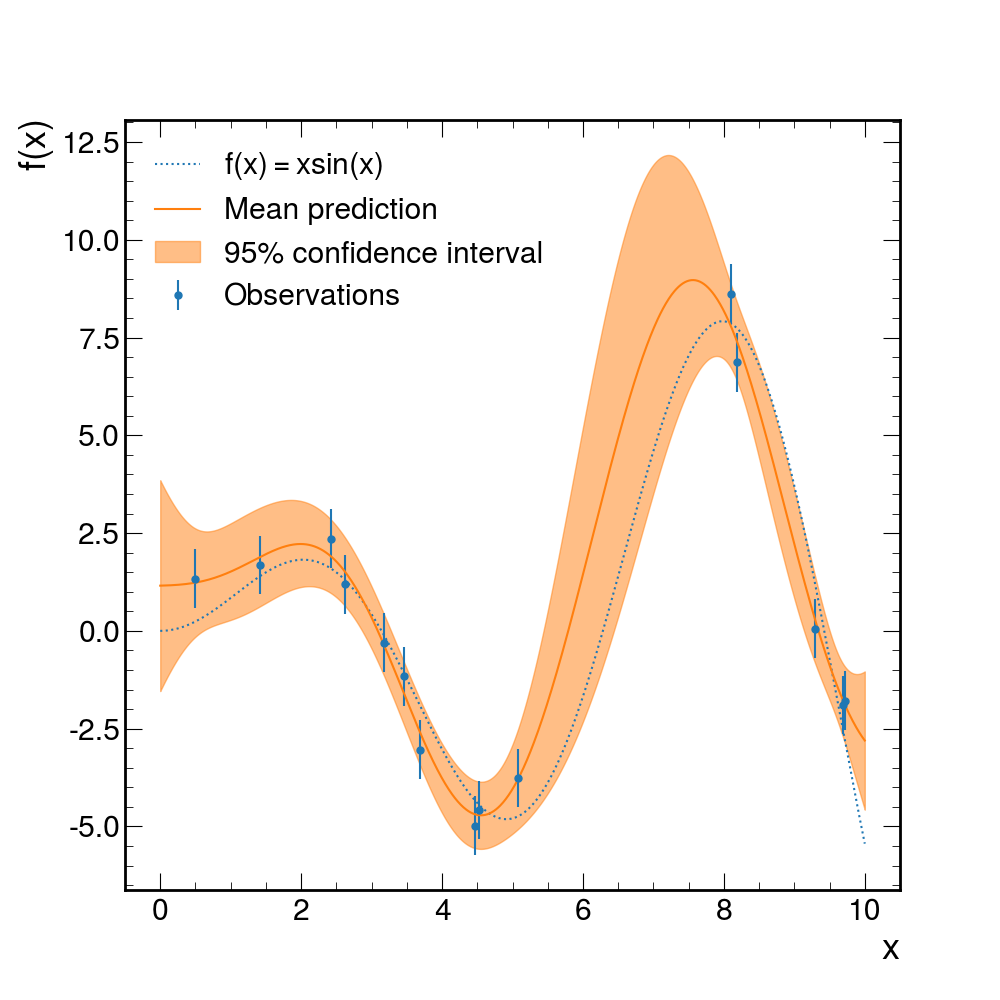
\includegraphics[width=8.0cm]{imgs/rbf.png}
\caption{Prediction using GPR method with sklearn.}
\label{rbf}
\end{figure}

According to figure \ref{rbf} predition error is relatively minimum in the region $2. < x < 4.$. This is because we have more observations in that region hence the small predition error. In the region $6. < x < 8.$ we have a relative large error because we have very few observations to make a prediction. This will cause the large prediction error.

In RBF kernel class length scale and length scale bounds are the two parameters we can used to optimize in the \href{https://scikit-learn.org/stable/modules/generated/sklearn.gaussian_process.kernels.RBF.html}{GPR}. Some of the common parameter we can optimize in GPR class is kernel, alpha value added to the diagonal of the kernel in the training, optimizer and number of restarts of the optimizer. More details about this class can be found in \verb|sklearn| \href{https://scikit-learn.org/stable/modules/generated/sklearn.gaussian_process.GaussianProcessRegressor.html} {documentation}. Some of the in build kernels is given in their \href{https://scikit-learn.org/stable/modules/gaussian_process.html#kernels-for-gaussian-processes}{documentation}.

Some disadvantages of the Gaussian process include \cite{scikit-learn};

\begin{itemize}
\item They are not sparse, i.e., they use the whole samples/features information to perform the prediction.
\item They lose efficiency in high dimensional spaces – namely when the number of features exceeds a few dozens.
\end{itemize}


\printbibliography

\end{document}
